\documentclass[crop,border={0pt 0 0 0},tikz]{standalone}
\usetikzlibrary{backgrounds,decorations.markings}
\tikzset{>=latex}
\tikzset{->-/.style={decoration={
  markings,
  mark=at position .5 with {\arrow{>}}},postaction={decorate}}}
\begin{document}
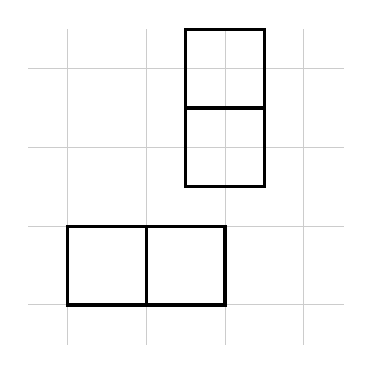
\begin{tikzpicture}
    
    \draw [step=1, line cap = rect, gray!40] (0.5,0.5) grid (4.5,4.5);
    

    \draw[black, line cap=rect, very thick] (2.5,2.5) rectangle (3.5,3.5);
    \draw[black, line cap=rect, very thick] (2.5,3.5) rectangle (3.5,4.5);

    \draw[black, line cap=rect, very thick] (1,1) rectangle (2,2);
    \draw[black, line cap=rect, very thick] (2,1) rectangle (3,2);


\end{tikzpicture}
\end{document}
